\documentclass[a4paper, fleqn]{article}
\usepackage{enumitem}
\usepackage{amsmath, amssymb}
\usepackage{xstring}
\usepackage{graphicx} % For including figures
\graphicspath{{./figs/}} % Path to figures
\usepackage[labelformat=empty]{caption} % To remove figure labels
% Set engineering notation
\providecommand{\sci}[1]{\protect\ensuremath{\times 10^{\StrSubstitute[0]{#1}{e}{}}}}
\setlength{\parindent}{0pt} % Set paragraph indentation to zero

\begin{document}

\underline{\textbf{Tutorial 6: Shafts and Associated Elements}}
\vspace{10pt}

\section*{In-class activities}

\begin{enumerate}
    \item Find the maximumum bending moment from the figure.
    \begin{figure}[h]
        \centering
        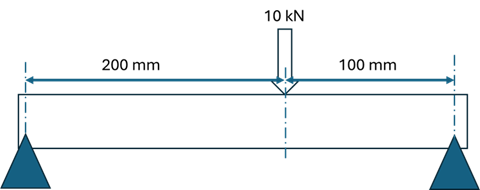
\includegraphics[width=0.5\textwidth]{t5-class1.png}
        \end{figure}
    \item  The key is fixed on the shaft with a key of dimension of 12 mm x 12 mm x 12 mm. Estimate the diameter of the shaft.
    \item  State the width and thickness of a square key for a shaft of diameter 80 mm. 
    \end{enumerate}


\section*{Theory}
\begin{enumerate}
    \item Define shaft's key and list two conditions that can affect the key's dimension.
    \item Explain the main function and application of a coupling
    \item List two types of pins used in shaft.
    \item Explain the function and application of spline
\end{enumerate}

\newpage

\section*{Calculations}

\textbf{Question 1}

A solid steel shaft with $S_y$= 250MPa, carries belt tensions vertically at pulley C, as shown in Figure below. Given diameter of pulley is 300mm, and a factor of safety of n=1.5, design the shaft according to the following failure criteria

\begin{enumerate}[label=(\roman*)]
    \item Maximum Shear Stress Theory
    \item Maximum Energy of Distortion Theory
\end{enumerate}

\begin{figure}[h]
    \centering
    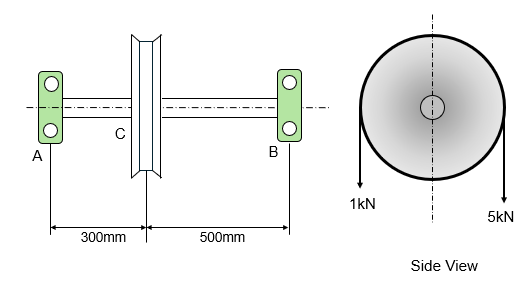
\includegraphics[width=0.75\textwidth]{t5-q1-1.png}
    \end{figure}

\vspace{10pt}
\textbf{Example Solution}
\vspace{10pt}

\textbf{Given Data:}

Steel shaft with $S_y$= 250MPa

Pulley diameter, d=300mm = 0.300mm

Pulley radius, r= d/2 = 0.150 m

Factor of safety, n=1.5

Belt tensions at pulley C: $T_1$= 5 kN, $T_2$= 1kN

\vspace{10pt}
i - Design the shaft (determine diameter) using Maximum Shear Stress Theory of failure

\textbf{Step 1:} Analyse belt tensions at pulley. Find torque and forces acting on the shaft.

\begin{equation*}
    \begin{aligned}
        T_c &= r(F_1 - F_2) \\
        &= 0.150(5000 - 1000) \\
        &= 600 Nm \\
    \end{aligned}
\end{equation*}

Total load at C, $F_C$ = $F_1$ + $F_2$ = 5 kN + 1 kN = 6 kN

\vspace{10pt}
\textbf{Step 2:} Calculate the reactions at the supports A and B

Draw the free body diagram of the shaft:

\begin{figure}[h]
    \centering
    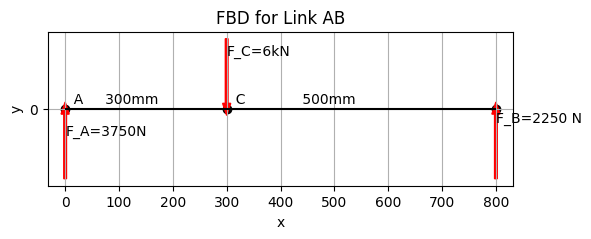
\includegraphics[width=0.75\textwidth]{t5-q1-2.png}
    \end{figure}

Taking moments about A to find reaction at B:

\begin{equation*}
    \begin{aligned}
        +\circlearrowleft \sum M_A &=0 \\
        -F_C(0.3)+F_B(0.8) &=0 \\
        -(6000)(0.3)+F_B(0.8) &=0 \\
        F_B &=2250 N \\
        +\uparrow \sum F_y=0 \\
        F_A  + F_B - F_C&=0 \\
        F_A + 2250- 6000  &=0 \\
        F_A &=3750 N \\        
    \end{aligned}
\end{equation*}


\textbf{Step 3:} Draw shear force and bending moment diagrams to find maximum bending moment.

\begin{figure}[h]
    \centering
    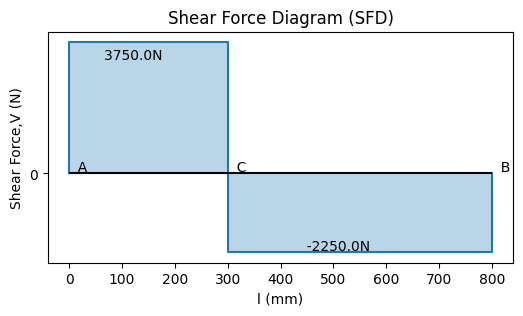
\includegraphics[width=0.75\textwidth]{t5-q1-3.png}
    \end{figure}

\newpage
\begin{figure}[h]
    \centering
    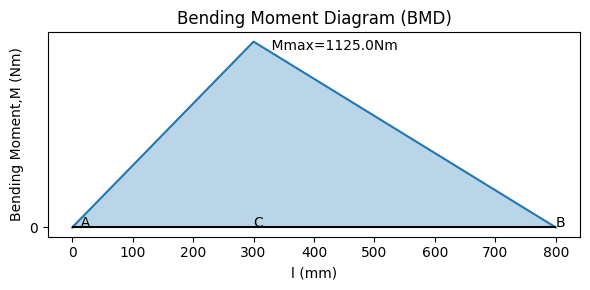
\includegraphics[width=0.75\textwidth]{t5-q1-4.png}
    \end{figure}

Maximum bending moment, $M_{max}$ = 1125 Nm

\vspace{10pt}
\textbf{Step 4:} Calculate the diameter of the shaft using Maximum Shear Stress Theory of failure.

i - Design the shaft (determine diameter) using Maximum Shear Stress Theory of failure
\vspace{10pt}
From Maximum Shear Stress Theory of failure:
\begin{equation*}
    \begin{aligned}
        \dfrac{S_y}{n} &= \frac{32}{\pi D^3} (M^2 + T^2)^ \frac{1}{2} \\
        D^3 &= \frac{32 n}{\pi S_y} (M^2 + T^2)^ \frac{1}{2} \\
        D^3 &= \frac{32 (1.5)}{\pi (250 \times 10^6)} \left[(1125)^2 + (600)^2\right]^{\frac{1}{2}} \\
        &= 7.7922 \times 10^{-5} m^3 \\
        D &= 0.04271 m = 42.7 mm \\
    \end{aligned}
\end{equation*}

The minimum diameter of the shaft is 43mm.

\vspace{10pt}
ii - Design the shaft (determine diameter) using Maximum Energy of Distortion Theory of failure
\vspace{10pt}
From Maximum Energy of Distortion Theory of failure:
\begin{equation*}
    \begin{aligned}
        \dfrac{S_y}{n} &= \frac{16}{\pi D^3} \left[ (M^2 + \frac{3}{4} T^2) \right]^{\frac{1}{2}} \\
        D^3 &= \frac{16 n}{\pi S_y} \left[ (M^2 + \frac{3}{4} T^2) \right]^{\frac{1}{2}} \\
        &= \frac{16 (1.5)}{\pi (250 \times 10^6)} \left[ (1125)^2 + \frac{3}{4}(600)^2 \right]^{\frac{1}{2}} \\
        &= 7.573 \times 10^{-5} m^3 \\
        D &= 0.04231 m = 42.3 mm \\
    \end{aligned}
\end{equation*}

The minimum diameter of the shaft is 43mm.

\newpage
\textbf{Question 2}

A shaft shown in the Figure Q2 moves at 16rpm to transmit 1kW power from pulley B to Pulley A. Design the shaft according to Maximum shear stress theory of failure Sy=550MPa and n=2.
\begin{figure}[h]
    \centering
    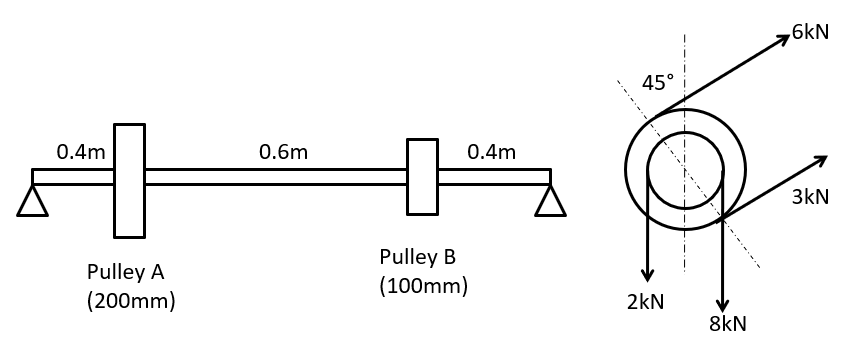
\includegraphics[width=0.75\textwidth]{t5-q2-1.png}
    \caption{Figure Q2}
    \end{figure}

\newpage
\textbf{Question 3}

Figure Q3 shows a shaft loaded with pulleys C and D, supported by bearings A and
B. The shaft transmits 70 kW of power at 1500 rpm to both pulleys. The diameters of
pulleys C and D are 150 mm and 100 mm, respectively. Meanwhile, the belt tension
ratios for pulley C and D are 2:1 and 3:2, respectively. The high-strength steel with a
yield stress of Sy=345 MPa is used for the shaft, with a safety factor of 2.5

\begin{enumerate}[label=(\roman*)]
    \item Determine the belt tension on pulley C and D.
    \item Determine the diameter of the shaft using maximum shear stress theory of failure.
    \item If the material of the shaft changes to 600 MPa of the yield stress, suggest the
    new diameter of the shaft.
\end{enumerate}

\begin{figure}[h]
    \centering
    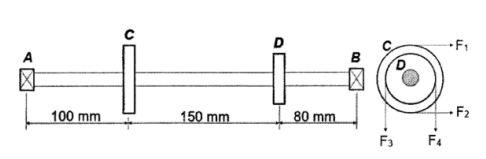
\includegraphics[width=0.75\textwidth]{t5-q3-1.png}
    \caption{Figure Q3}
\end{figure}

\newpage
\textbf{Question 4}

The layout of a shaft carrying two pulleys A and C and supported by two bearings B and D is shown Figure Q4.
The shaft transmits power at 360 rpm from pulley A to pulley C. The diameter of pulley A and C are 200 mm and 300 mm respectively. The belt tensions act horizontally at pulley C and the ratio of belt tension on the tight side to the slack side is 2.5:1. The shaft is made of plain carbon steel with a yield strength of 280MPa and the factor of safety is 2.

\begin{enumerate}[label=(\roman*)]
    \item Determine the belt tensions on pulley C.
    \item Determine the diameter of the shaft using maximum shear stress theory of failure.
    \item What is the new diameter of the shaft if the factor of safety is increased to 3.
\end{enumerate}
\begin{figure}[h]
    \centering
    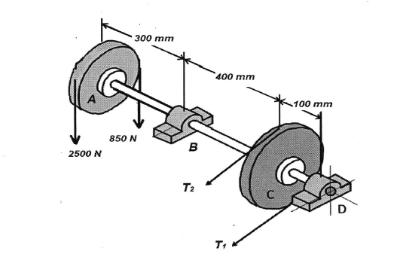
\includegraphics[width=0.75\textwidth]{t6-q4-1.png}
    \caption{Figure Q4}
\end{figure}

\newpage

\textbf{Answer}

\textbf{Q2}
d= 45mm

\textbf{Q3}

\begin{enumerate}[label=(\roman*)]
    \item T$_1$= 11883.46 N, T$_2$= 5941.73 N, T$_3$= 26737.8 N, T$_4$= 17825.2 N
    \item d= 59mm
    \item d= 49mm
\end{enumerate}

\textbf{Q4}
\begin{enumerate}[label=(\roman*)]
    \item T$_1$= 1834.8 N, T$_2$= 733.9 N
    \item d= 42mm
    \item d= 48mm
    \end{enumerate}

\end{document}